\documentclass{chi2012}
\newcommand{\tab}{\hspace*{2em}}
\usepackage{times}
\usepackage{graphics}
\usepackage{color}
\usepackage[pdftex]{hyperref}
\hypersetup{%
pdftitle={Using Diversity within the Crowd},
pdfauthor={Durga M. Kandasamy, Kristal Curtis, Armando Fox, David Patterson},
pdfkeywords={Crowdsourcing, Diversity, Image labeling},
bookmarksnumbered,
pdfstartview={FitH},
colorlinks,
citecolor=black,
filecolor=black,
linkcolor=black,
urlcolor=black,
breaklinks=true,
}
\newcommand{\comment}[1]{}
\definecolor{Orange}{rgb}{1,0.5,0}
\newcommand{\todo}[1]{\textsf{\textbf{\textcolor{Orange}{[[#1]]}}}}

\pagenumbering{arabic}  % Arabic page numbers for submission.  Remove this line to eliminate page numbers for the camera ready copy

\begin{document}
% To make various LaTeX processors do the right thing with page size.
\special{papersize=8.5in,11in}
\setlength{\paperheight}{11in}
\setlength{\paperwidth}{8.5in}
\setlength{\pdfpageheight}{\paperheight}
\setlength{\pdfpagewidth}{\paperwidth}

% Use this command to override the default ACM copyright statement
% (e.g. for preprints). Remove for camera ready copy.
% \toappear{Submitted for review to CHI 2012.}

\title{Using Diversity within the Crowd}
\numberofauthors{4}
\author{
  \alignauthor Durga M. Kandasamy\\
    \affaddr{AMP Lab at UC Berkeley}\\
    \affaddr{465 Soda Hall, MC 1776\\
    		Berkeley,CA 94720-1776}
    \email{durga.m.kandasamy@berkeley.edu}
  \alignauthor Kristal Curtis\\
    \affaddr{AMP Lab at UC Berkeley}\\
    \affaddr{465 Soda Hall, MC 1776\\
    		Berkeley,CA 94720-1776}
    \email{  kcurtis@eecs.berkeley.edu}
      \alignauthor Armando Fox\\
    \affaddr{AMP Lab at UC Berkeley}\\
    \affaddr{465 Soda Hall, MC 1776\\
    		Berkeley,CA 94720-1776}
    \email{fox@eecs.berkeley.edu}
      \alignauthor David Patterson\\
    \affaddr{AMP Lab at UC Berkeley}\\
    \affaddr{465 Soda Hall, MC 1776\\
    		Berkeley,CA 94720-1776}
    \email{pattrsn@eecs.berkeley.edu}
}

\maketitle

\begin{abstract}
%\tab When attempting to efficiently solve problems, we often turn to experts. Though this is logical, experts are often unavailable or too costly. We believe that being more diverse in questioning could be beneficial in producing the best solution to the task at hand. Intuitively, by surveying a diverse population, there is the potential for less redundancy among the responses. We strive to combine responses from expert and general members of the crowd to produce the best results for an image labeling task. We found that using a diverse group, we could approach (and sometimes exceed) the performance of the expert group while achieving better throughput for a lesser cost. 
Crowdsourcing holds great promise for enabling many applications which are difficult to accomplish automatically.  However, many people grapple with how to pose their tasks in a way that will enable them to obtain the desired output.  This difficulty lies not only in framing the task but also in determining which members of the crowd should be recruited to complete the task.  In some cases, expert knowledge is desired; however, expert input may not be available in the desired quantity given the time and cost constraints of the problem.  When this is the case, it would be beneficial to augment the expert input that is available with input from members of the general population if this would lead to an improved outcome.  We believe that reduced reliance on experts (bolstered by diversity) will in some cases lead to acceptable performance while reducing cost and latency.  We explored this approach in the context of an image labeling task on Mechanical Turk.  In this work, we show that we are able to approach or exceed the performance of an expert group while reducing our reliance on experts by incorporating non-expert responses. 
\end{abstract}

\keywords{Crowdsourcing, Diversity, Image labeling} 

\category{H.5.2}{Information Interfaces and Presentation}{Miscellaneous}[Optional sub-category]

\terms{
}

\section{Introduction}

%\tab Finding a competent group of workers is crucial in order to successfully complete a given task. Intuitively, expert input is more valuable than that of the general population.  However, experts may be unavailable or too costly. The necessity of an expert's opinion is task specific- tasks which rely on a higher level of understanding in a certain field require a certain level of expertise, while tasks regarding general knowledge can benefit greatly from diversity, since individuals bring in different perspectives in commonly known subject areas. In this work, we explore the idea that using a diverse group for tasks such as image labeling can result in performance meeting or exceeding the level of the experts while being more available and budget-friendly.

%\tab To analyze this problem, we used Amazon Mechanical Turk\footnote{www.mturk.com}, an internet marketplace that allows programmers (Requesters) to access human intelligence (Workers) for problems that are currently difficult for computers. 

%\tab Most recently, Mechanical Turk introduced the \textit{Masters} distinction for two types of tasks, Photo Moderation and Categorization. According to the MTurk Blog, using a Photo Moderation Qualification would be best if the task involves reviewing a photo or identifying content in a photo, and the Categorization Qualification could be used for tasks which involve categorizing data \footnote{http://mechanicalturk.typepad.com/blog/2011/06/get-better-results-with-less-effort-with-mechanical-turk-masters-.html}.


Finding a competent group of workers is crucial in order to successfully complete a given crowdsourcing task.  Intuitively, expert input is more valuable than that of the general population.  However, experts may be unavailable or too costly.  

Consider a given task.  There is likely to be some minimum amount of related knowledge than any worker must possess before they can make progress on the problem (e.g., in order to participate in proofreading a text written in English, a worker should be able to speak English).  Intuitively, you would expect that you could get the best performance by turning to a group of subject experts (in our example, a group of experts might consist of English teachers).  Our goal is to explore whether it is possible to approximate the performance of the expert group with a diverse group.  For our purposes, a diverse group is defined as one that consists of experts as well as non-experts.  A non-expert is a person who possesses the minimum amount of subject knowledge required but is less competent than an expert at performing tasks like the one given.  A diverse group that produces work of equivalent quality as that of an expert group is preferable since it reduces the dependency on experts; solutions using fewer experts cost less and complete more quickly.

To analyze this problem, we used Amazon Mechanical Turk\footnote{www.mturk.com}, an internet marketplace that allows task providers (\textit{requesters}) to access human intelligence (\textit{workers}) for problems that are currently difficult for computers alone.
Mechanical Turk recently introduced the \textit{Masters} qualification to recognize Turkers who have consistently exhibited excellent performance.
% could explain Masters a bit more here -- look at blog post
The Masters qualification is available for two types of tasks: Photo Moderation and Categorization.  
According to the MTurk blog, workers who have been recognized as Photo Moderation Masters perform well at tasks that involve reviewing photos or identifying their contents.  % verify this

\tab In what follows, workers with Masters distinctions would be classified as experts. We expect the Photo Moderation Masters to perform better at our image labeling task, though there is some overlap with the Categorization Masters since workers are also expected to categorize the image contents. A diverse group of responses is created by mixing the responses of Masters qualified workers with general workers, while a non-diverse collection of responses consists of those strictly from Masters workers, or strictly from general workers.

\section{Related Work}
\tab In \cite{wisdomOfCrowds}, Surowiecki explores the benefits of diversity, referring to an experiment in \cite{HongPage:2000} where the authors formed several sets of agents, each consisting of 10-20 members. Each agent had a varying skill set, and together they were asked to solve a given problem. Page concluded that groups which consisted of a mix of ``smart'' and ``not-so-smart'' agents did a better job than groups consisting of only ``smart'' agents \cite{HongPage:2000}. Surowiecki notes that having diversity within a group is useful since it adds perspectives that would not have otherwise been contributed and reduces the effect of some negative qualities which may come with group decision making.

\tab The authors of \cite{ShahafHorvitz:2010} develop the idea of finding the best ``coalition'' to work on a task. Each agent within the group has a corresponding ability vector which represents its capabilities along several dimensions of interest. Finding an ability vector is a hard problem; in \cite{ShahafHorvitz:2010}, the authors required workers to complete a self-assessment of their competence. In our work, we decided to make use of the Masters qualification as a proxy. 

\section{Experimental Setup}
\tab In the Human Intelligence Task (HIT), workers were given a women's clothing image (Figure 1) and were asked to (1) identify the number of items of clothing appearing in the image, and (2) describe these items of clothing. 

\begin{figure}
\centering
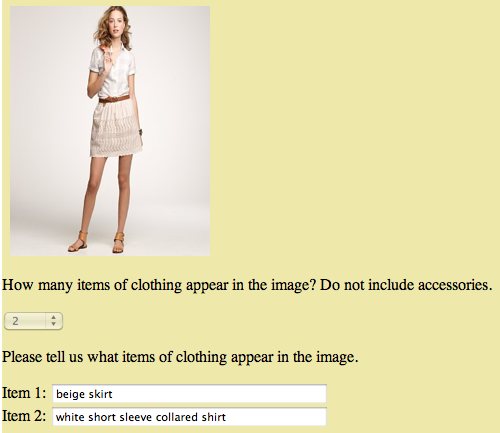
\includegraphics[width=0.9\columnwidth]{Figure1}
\caption{An example HIT posted on Mechanical Turk}
\label{fig:figure1}
\end{figure}

\tab To test their correctness in labeling the items of clothing, workers were asked to be as descriptive as possible. Each experiment run had 10 unique images, allowing a minimum of 10 unique workers to complete the tasks in each run. In order to observe the effect of using an expert group versus a diverse group, the experiment was carried out over the course of three runs. For each HIT over all three runs, Workers could earn \$0.10. However due to the fact that Mechanical Turk collects a fee of 20\% of the assignment reward for the Masters distinction, the total cost for the Photo Moderation and Categorization runs were greater than that of the General run. In the first run, only Photo Moderation Masters qualified workers could work on the posted HITs. In the next run, all workers, regardless of whether they had a Masters distinction were allowed to work on the HITs. In the final run, workers were restricted such that only those with the Categorization Masters distinction could work on the posted tasks. 

\section{Results}
\tab In both the Photo Moderation and Categorization runs, workers were required to have an expert distinction, while in the General run all Mechanical Turk Workers were allowed to complete the HITs. When checking for worker overlap among the three experiment runs, we noticed only one worker had submitted to both the Photo Moderation and the General run. While conducting the experiments, a distinct difference in throughput was also noticed. Understandably, the General run took the least amount of time to reach completion- around two hours. Since all Mechanical Turk workers qualified for this run, these HITs were rapidly completed. While the Photo Moderation run took around 18 hours to be completed, the Categorization run took 9 days to successfully run to completion. Once all the responses were received, they were reviewed manually to correct spelling differences (''color'' versus ''colour'') as well as to make similar labels (''pant'' versus ''pants'') consistent. This allowed us to begin analyzing the data.

\tab Responses from each of the runs were parsed into single words, or tokens. When comparing how often workers within a single experiment use the same tokens to describe the image, we found most workers to be original in their labeling. In Figure 2, we show the graph for an arbitrary image, Image 3. Though the expert runs had the most number of single occurrence tokens, tokens with the most number of occurrences also occurred in the expert runs. This hints towards a redundancy amongst the expert group.
 
 \begin{figure}
\centering
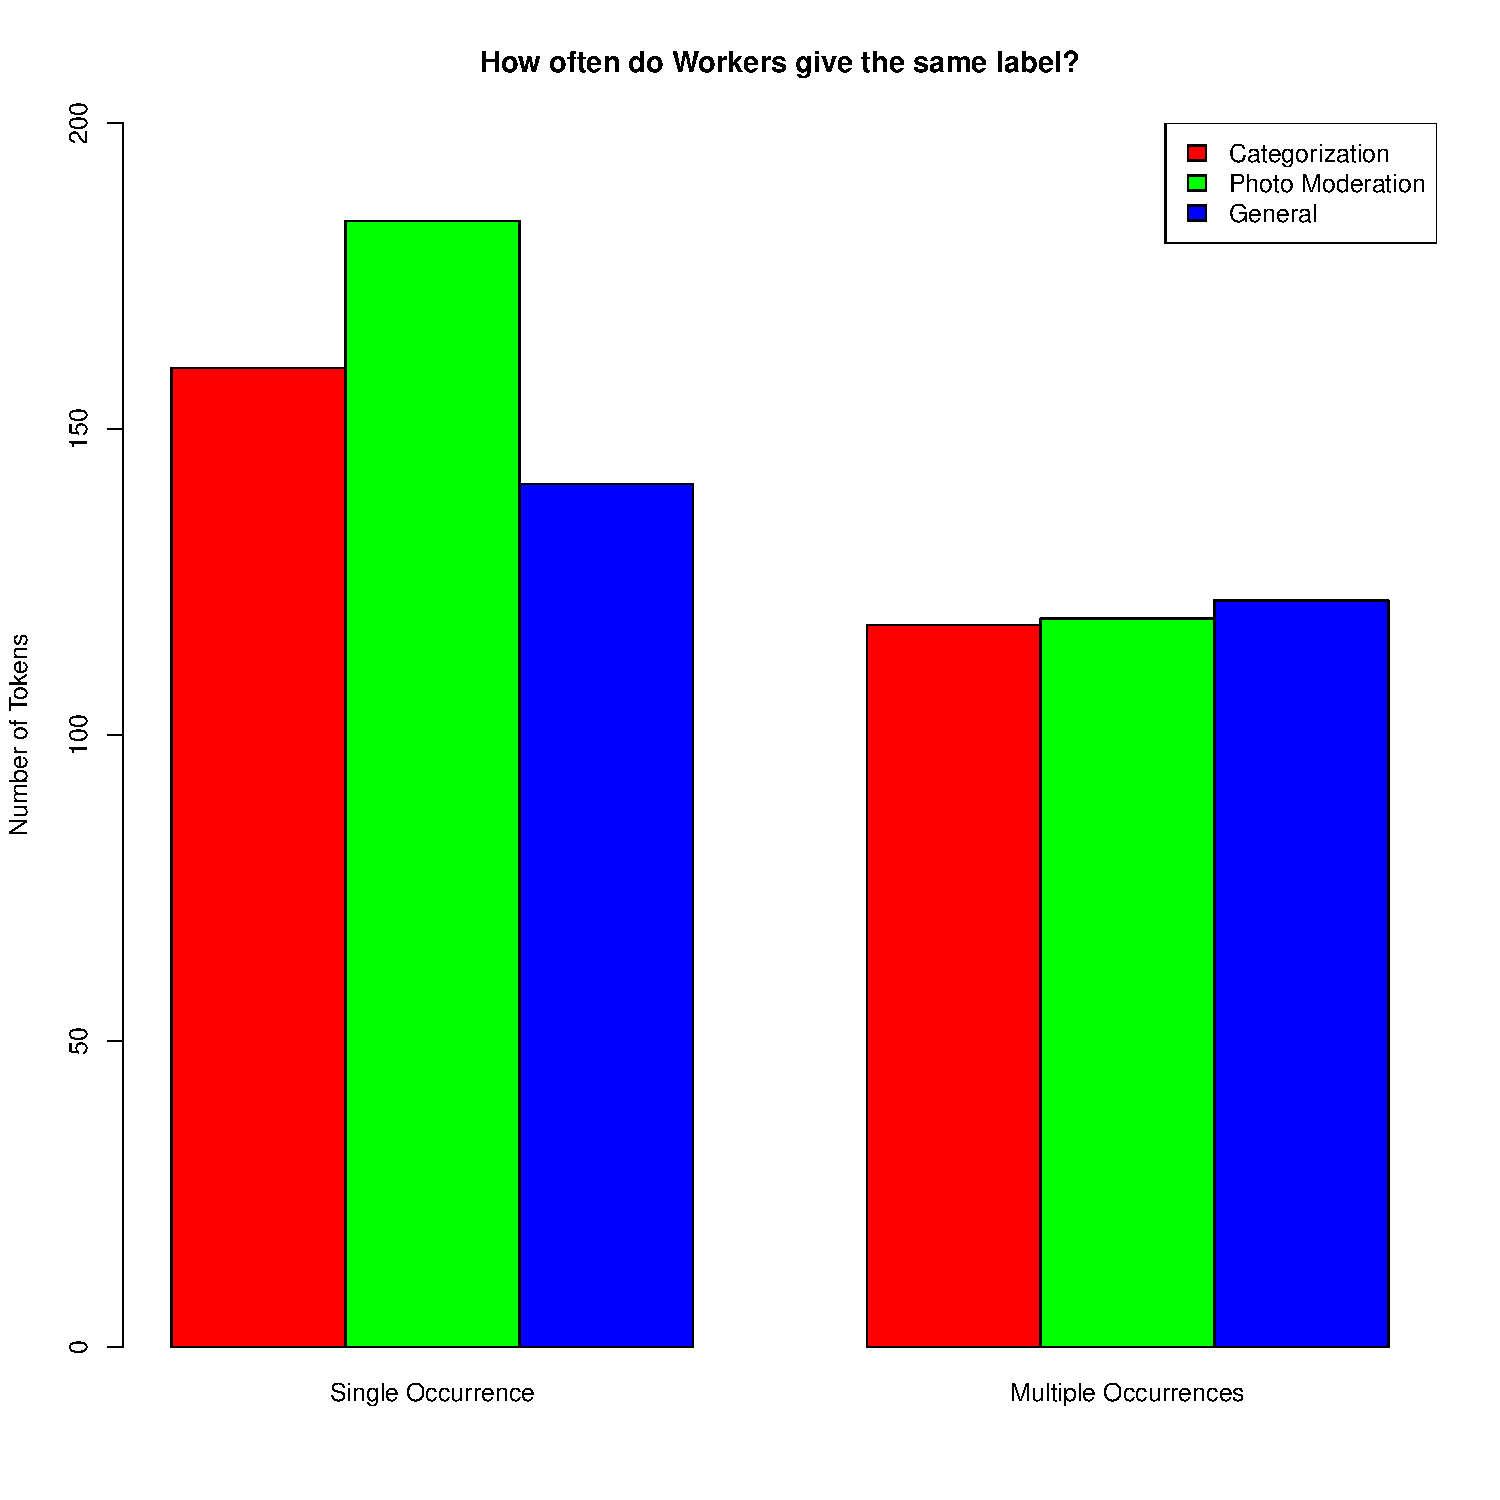
\includegraphics[width=0.9\columnwidth]{extendedAbstractOccurrence}
\caption{As can be observed in the graph above, workers with a Photo Moderation Masters distinction gave the most original responses. Most of their tokens only had a single occurrence each. At the same time, all three categories of workers had approximately the same number of tokens which had multiple occurrences. }
\label{fig:figure1}
\end{figure}
 
\tab Using these three experiment runs, a more diverse group of worker responses was created. Using a randomly generated set of indices, we selected worker responses among the three groups. These responses were grouped together to create the mix group of responses. Similar to the original sets of responses, this new set  was parsed into single word tokens used to describe each image. From these tokens, the top tokens, tokens which were used in at least five of the 10 responses for each image, were extracted. We established the ground truth by first individually reviewing and labeling the images we were also asking the Mechanical Turk workers to consider, then taking the union of our responses. Accuracy was measured by comparing how many of the top tokens within a set also appeared in the established ground truth. Our ground truth was limited in that synonyms of ground truth words were excluded from qualifying as a correct response. Using the number of tokens that matched and the total number of tokens in the ground truth, a score was calculated for each image as follows:
\\
\\
\begin{math}
Image \ Score=\frac{|Matching \ top \ tokens|}{|Ground \ truth \ tokens|}
\end{math}
\\
\\
\tab After creating a simple diverse group with a ratio of 50-50 from Photo Moderation-Categorization, we were interested in seeing what effect altering the mix ratio would have on the calculated score. We decided to create a group with a ratio of 40-30-30 from Photo Moderation-Categorization-General.   

 \begin{figure}
\centering
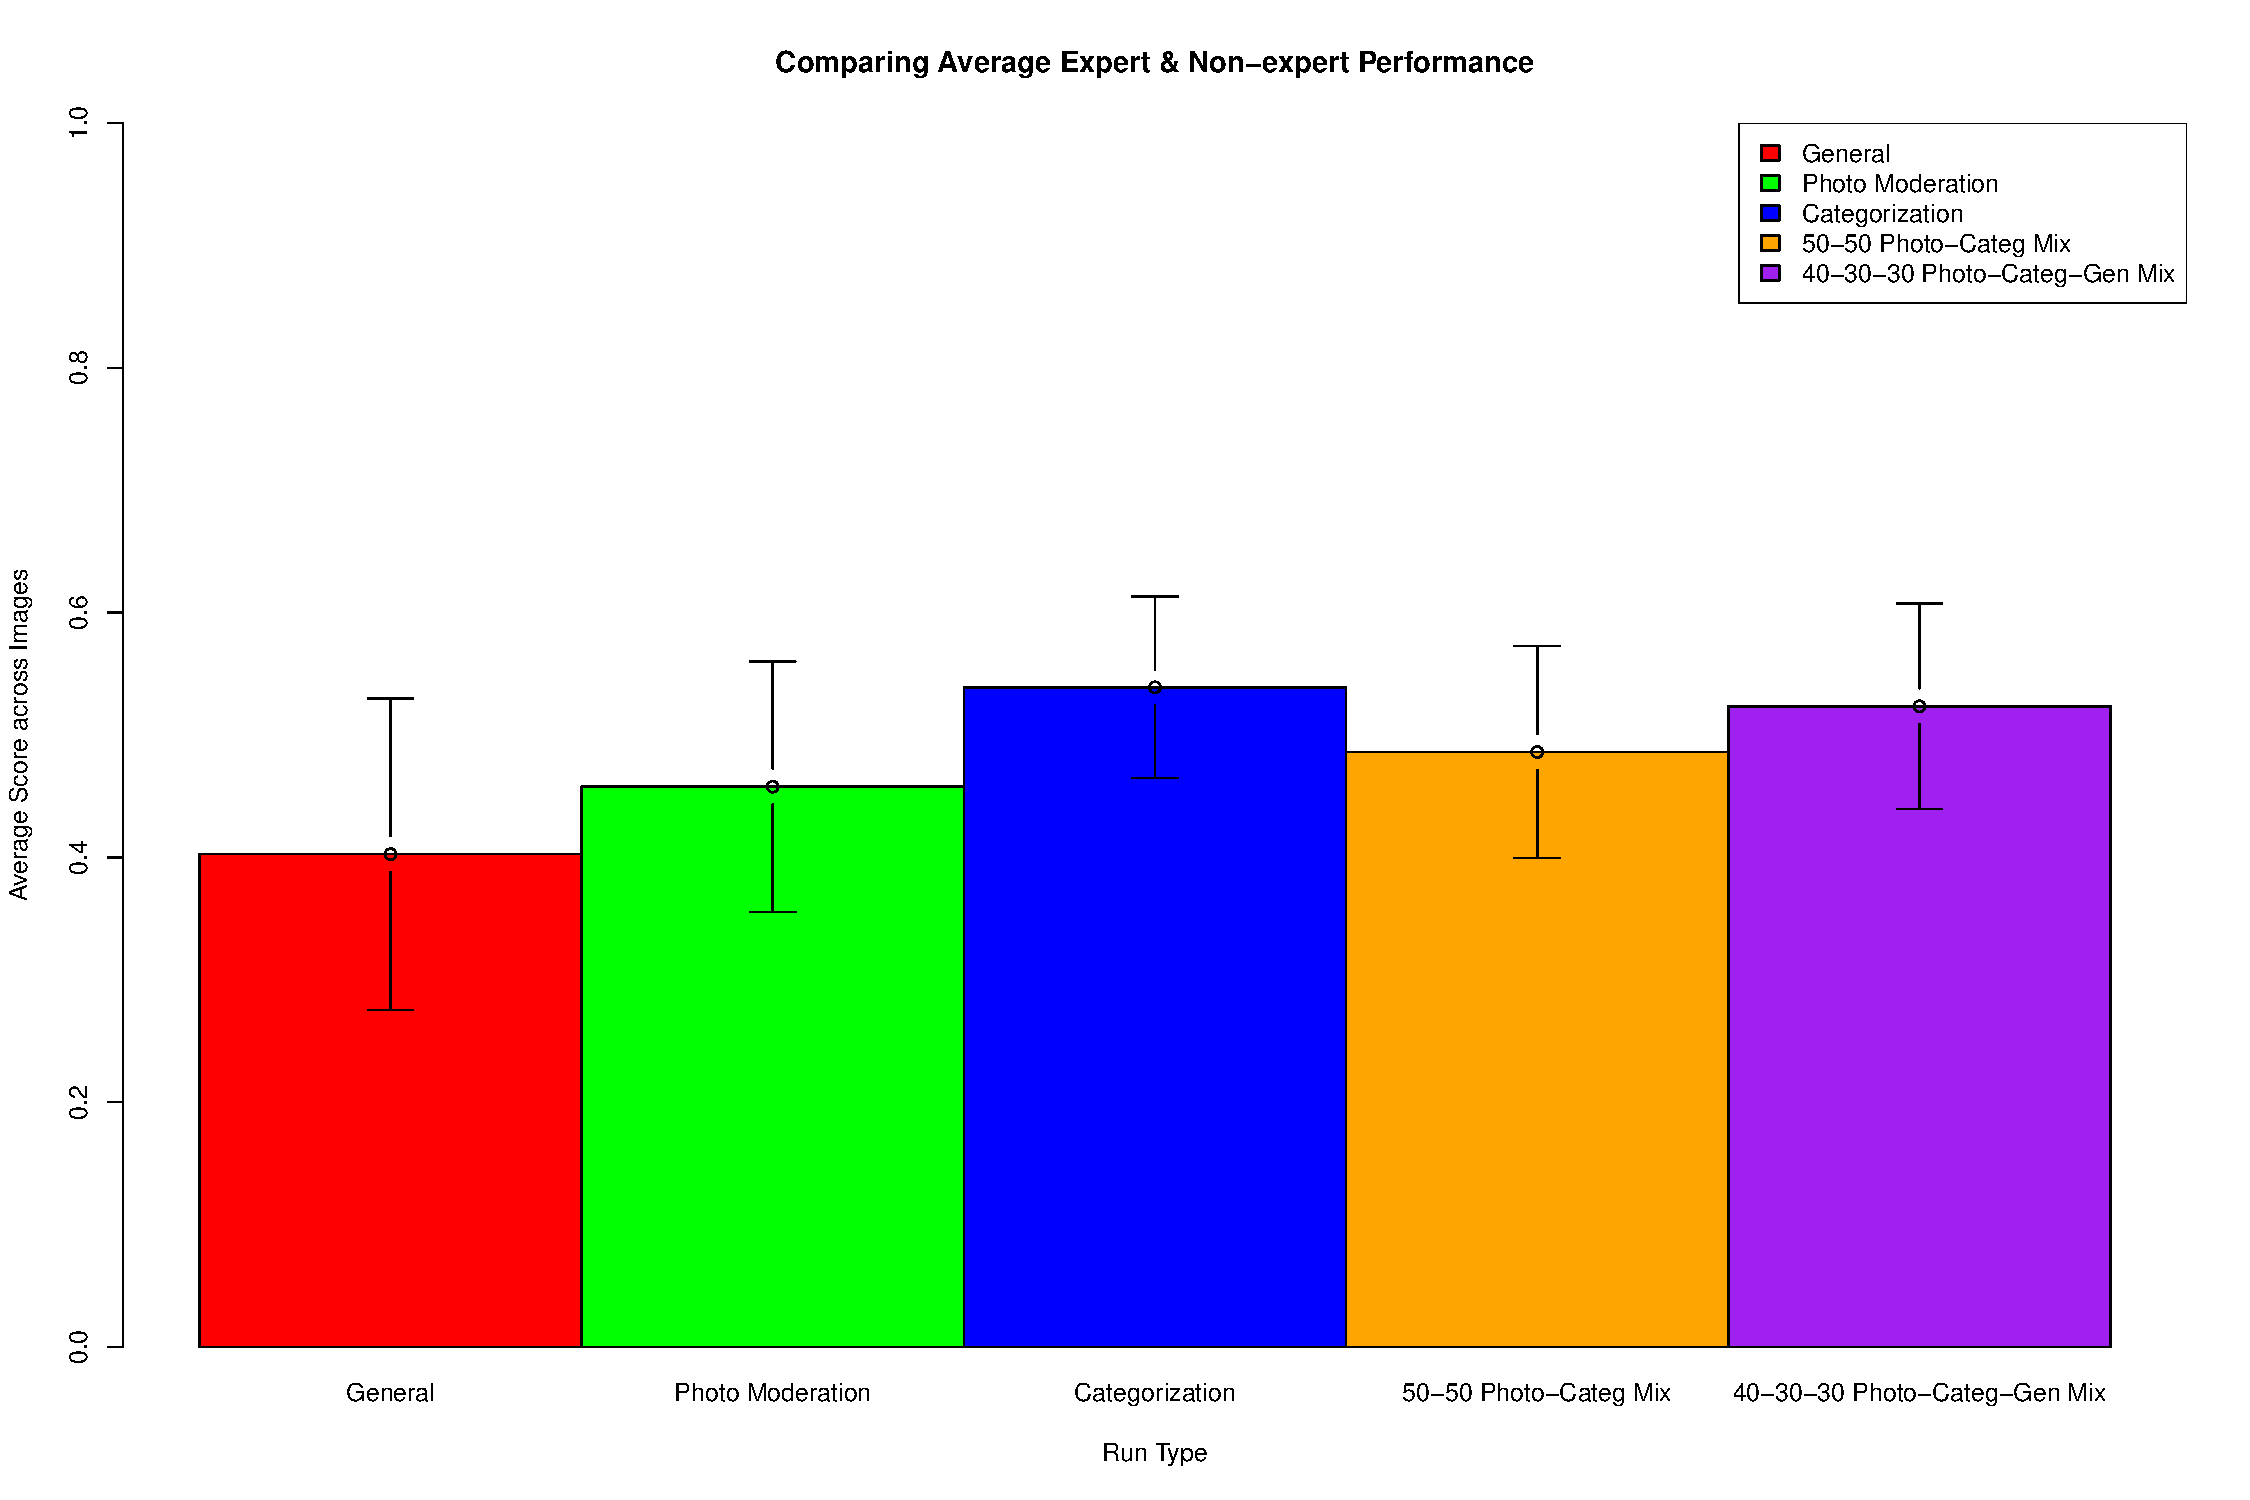
\includegraphics[width=0.9\columnwidth]{averageScores}
\caption{From this graph, it can be deduced that it is plausible to create a diverse mix of workers whose score value is close to that of a Master's. Tuning the ratio of worker types in the diverse group could potentially give an even more improved score. }
\label{fig:figure1}
\end{figure} 

\tab As hypothesized, having a diverse group seems to allow for a greater variety of responses, producing a higher score. This proves to be valuable since Mechanical Turk charges more money for Masters qualified experiments. Finding an optimal ratio of expert and general would save money, as well as time, since as we noted earlier, the throughput for the General run was higher than that of those with Masters distinction.

 \begin{figure}
\centering
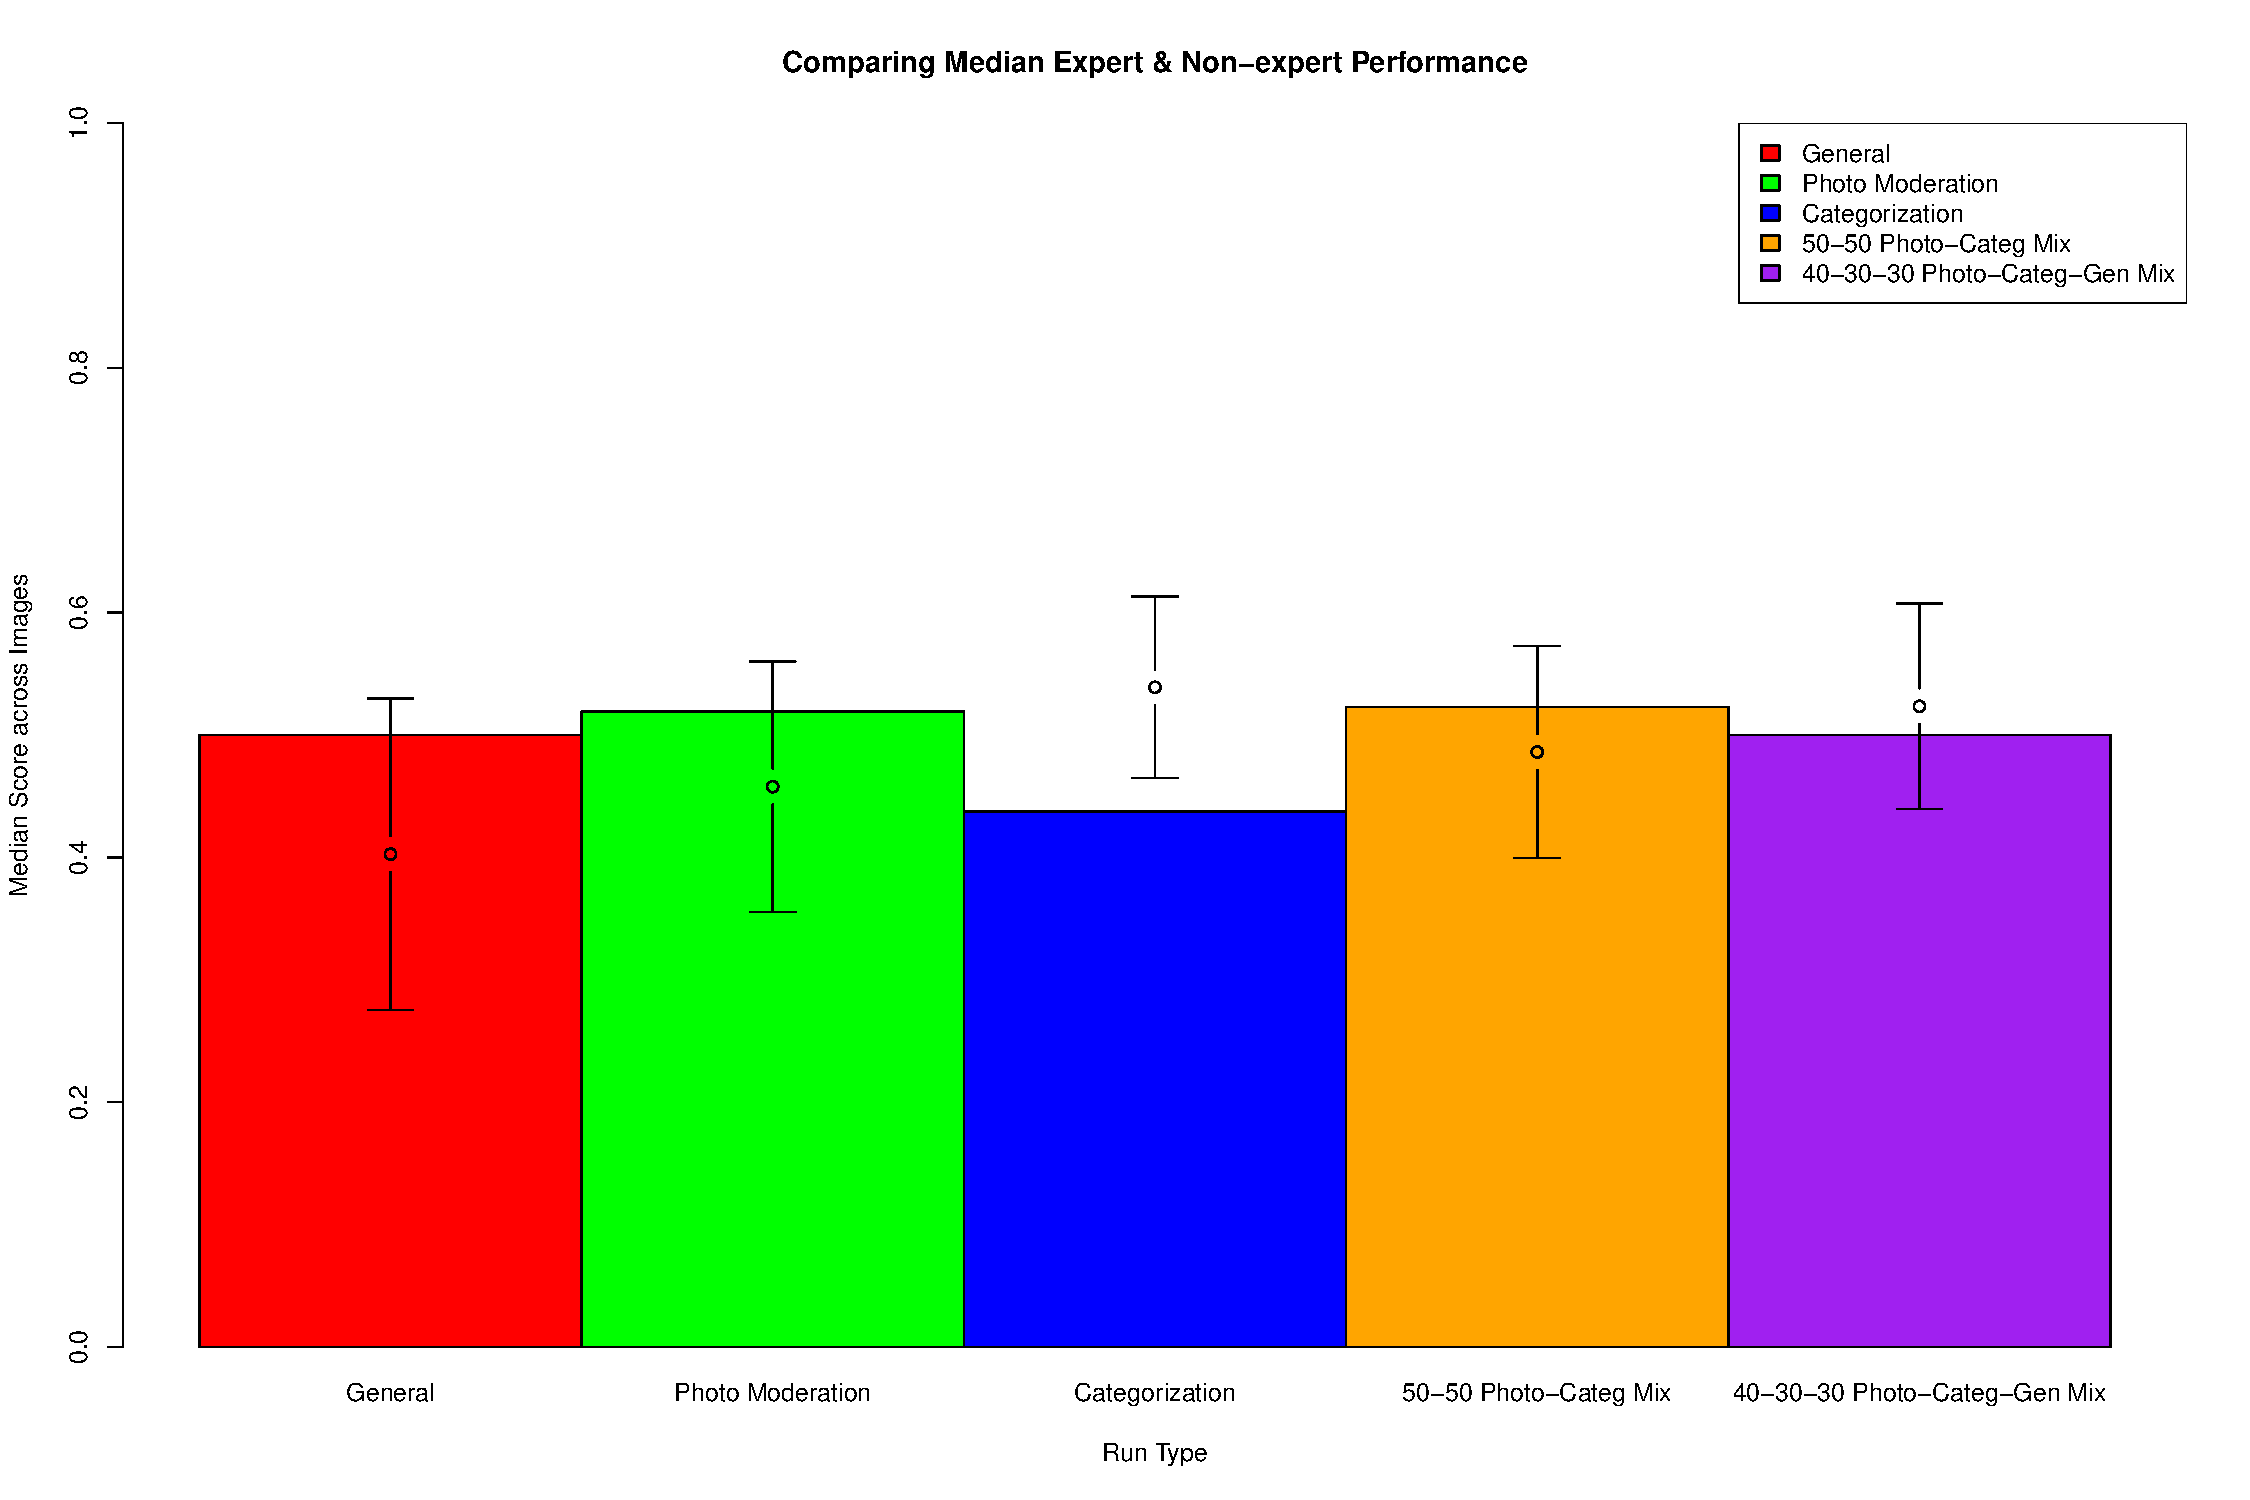
\includegraphics[width=0.9\columnwidth]{medianScores}
\caption{While the mean score of the Categorization workers was the greatest, taking the median of the group shows that the Photo Moderation Masters outperforms the Categorization Masters. Still however, the diverse mix of workers performs as well as the Masters.}
\label{fig:figure1}
\end{figure} 

\section{Conclusion}

\tab We see that at times a diverse group of workers, with the correct ratio of expert to general, may perform better than a group of strictly expert workers. This shows that there are advantages to using a diverse group consisting of a mix of general and expert members. It would provide an higher throughput, while still being cost effective. We plan to continue working on this problem by creating a series of groupings for each ratio type and aggregating scores, rather than only using the scores collected from one grouping for each ratio. We hope this will give us a more definite score value for each ratio of expert to general workers. 

\balancecolumns % add only when the article is done

% Don't forget to balance the columns with 
% \balancecolumns
% simple but not very good, or
% add \usepackage{balance} at the beginning and add
% \balance 
\bibliographystyle{acm-sigchi}
\bibliography{papers}

\end{document}
